\documentclass[journal]{IEEEtran}
\usepackage[numbers]{natbib}
\usepackage{url}
\usepackage{graphicx}
\usepackage{amsmath}
\usepackage{color}

%-- some setups
\newcommand{\ie}{i.e.\ }
\newcommand{\eg}{e.g.\ }
\newcommand{\Reffig}[1]{Fig.~\ref{#1}}
\newcommand{\Refsec}[1]{Sec.~\ref{#1}}
\newcommand{\Reftab}[1]{Tab.~\ref{#1}}
\newcommand{\COMMENT}[1]{\textcolor{red}{#1}}
%
% If IEEEtran.cls has not been installed in to the LaTeX system files,
% manually specify the path to it like:
% \documentclass[journal]{../sty/IEEEtran}





% Some very useful LaTeX packages include:
% (uncomment the ones you want to load)


% *** MISC UTILITY PACKAGES ***
%
%\usepackage{ifpdf}
% Heiko Oberdiek's ifpdf.sty is very useful if you need conditional
% compilation based on whether the output is pdf or dvi.
% usage:
% \ifpdf
%   % pdf code
% \else
%   % dvi code
% \fi
% The latest version of ifpdf.sty can be obtained from:
% http://www.ctan.org/pkg/ifpdf
% Also, note that IEEEtran.cls V1.7 and later provides a builtin
% \ifCLASSINFOpdf conditional that works the same way.
% When switching from latex to pdflatex and vice-versa, the compiler may
% have to be run twice to clear warning/error messages.






% *** CITATION PACKAGES ***
%
%\usepackage{cite}
% cite.sty was written by Donald Arseneau
% V1.6 and later of IEEEtran pre-defines the format of the cite.sty package
% \cite{} output to follow that of the IEEE. Loading the cite package will
% result in citation numbers being automatically sorted and properly
% "compressed/ranged". e.g., [1], [9], [2], [7], [5], [6] without using
% cite.sty will become [1], [2], [5]--[7], [9] using cite.sty. cite.sty's
% \cite will automatically add leading space, if needed. Use cite.sty's
% noadjust option (cite.sty V3.8 and later) if you want to turn this off
% such as if a citation ever needs to be enclosed in parenthesis.
% cite.sty is already installed on most LaTeX systems. Be sure and use
% version 5.0 (2009-03-20) and later if using hyperref.sty.
% The latest version can be obtained at:
% http://www.ctan.org/pkg/cite
% The documentation is contained in the cite.sty file itself.






% *** GRAPHICS RELATED PACKAGES ***
%
\ifCLASSINFOpdf
  % \usepackage[pdftex]{graphicx}
  % declare the path(s) where your graphic files are
  % \graphicspath{{../pdf/}{../jpeg/}}
  % and their extensions so you won't have to specify these with
  % every instance of \includegraphics
  % \DeclareGraphicsExtensions{.pdf,.jpeg,.png}
\else
  % or other class option (dvipsone, dvipdf, if not using dvips). graphicx
  % will default to the driver specified in the system graphics.cfg if no
  % driver is specified.
  % \usepackage[dvips]{graphicx}
  % declare the path(s) where your graphic files are
  % \graphicspath{{../eps/}}
  % and their extensions so you won't have to specify these with
  % every instance of \includegraphics
  % \DeclareGraphicsExtensions{.eps}
\fi
% graphicx was written by David Carlisle and Sebastian Rahtz. It is
% required if you want graphics, photos, etc. graphicx.sty is already
% installed on most LaTeX systems. The latest version and documentation
% can be obtained at: 
% http://www.ctan.org/pkg/graphicx
% Another good source of documentation is "Using Imported Graphics in
% LaTeX2e" by Keith Reckdahl which can be found at:
% http://www.ctan.org/pkg/epslatex
%
% latex, and pdflatex in dvi mode, support graphics in encapsulated
% postscript (.eps) format. pdflatex in pdf mode supports graphics
% in .pdf, .jpeg, .png and .mps (metapost) formats. Users should ensure
% that all non-photo figures use a vector format (.eps, .pdf, .mps) and
% not a bitmapped formats (.jpeg, .png). The IEEE frowns on bitmapped formats
% which can result in "jaggedy"/blurry rendering of lines and letters as
% well as large increases in file sizes.
%
% You can find documentation about the pdfTeX application at:
% http://www.tug.org/applications/pdftex





% *** MATH PACKAGES ***
%
%\usepackage{amsmath}
% A popular package from the American Mathematical Society that provides
% many useful and powerful commands for dealing with mathematics.
%
% Note that the amsmath package sets \interdisplaylinepenalty to 10000
% thus preventing page breaks from occurring within multiline equations. Use:
%\interdisplaylinepenalty=2500
% after loading amsmath to restore such page breaks as IEEEtran.cls normally
% does. amsmath.sty is already installed on most LaTeX systems. The latest
% version and documentation can be obtained at:
% http://www.ctan.org/pkg/amsmath





% *** SPECIALIZED LIST PACKAGES ***
%
%\usepackage{algorithmic}
% algorithmic.sty was written by Peter Williams and Rogerio Brito.
% This package provides an algorithmic environment fo describing algorithms.
% You can use the algorithmic environment in-text or within a figure
% environment to provide for a floating algorithm. Do NOT use the algorithm
% floating environment provided by algorithm.sty (by the same authors) or
% algorithm2e.sty (by Christophe Fiorio) as the IEEE does not use dedicated
% algorithm float types and packages that provide these will not provide
% correct IEEE style captions. The latest version and documentation of
% algorithmic.sty can be obtained at:
% http://www.ctan.org/pkg/algorithms
% Also of interest may be the (relatively newer and more customizable)
% algorithmicx.sty package by Szasz Janos:
% http://www.ctan.org/pkg/algorithmicx




% *** ALIGNMENT PACKAGES ***
%
%\usepackage{array}
% Frank Mittelbach's and David Carlisle's array.sty patches and improves
% the standard LaTeX2e array and tabular environments to provide better
% appearance and additional user controls. As the default LaTeX2e table
% generation code is lacking to the point of almost being broken with
% respect to the quality of the end results, all users are strongly
% advised to use an enhanced (at the very least that provided by array.sty)
% set of table tools. array.sty is already installed on most systems. The
% latest version and documentation can be obtained at:
% http://www.ctan.org/pkg/array


% IEEEtran contains the IEEEeqnarray family of commands that can be used to
% generate multiline equations as well as matrices, tables, etc., of high
% quality.




% *** SUBFIGURE PACKAGES ***
%\ifCLASSOPTIONcompsoc
%  \usepackage[caption=false,font=normalsize,labelfont=sf,textfont=sf]{subfig}
%\else
%  \usepackage[caption=false,font=footnotesize]{subfig}
%\fi
% subfig.sty, written by Steven Douglas Cochran, is the modern replacement
% for subfigure.sty, the latter of which is no longer maintained and is
% incompatible with some LaTeX packages including fixltx2e. However,
% subfig.sty requires and automatically loads Axel Sommerfeldt's caption.sty
% which will override IEEEtran.cls' handling of captions and this will result
% in non-IEEE style figure/table captions. To prevent this problem, be sure
% and invoke subfig.sty's "caption=false" package option (available since
% subfig.sty version 1.3, 2005/06/28) as this is will preserve IEEEtran.cls
% handling of captions.
% Note that the Computer Society format requires a larger sans serif font
% than the serif footnote size font used in traditional IEEE formatting
% and thus the need to invoke different subfig.sty package options depending
% on whether compsoc mode has been enabled.
%
% The latest version and documentation of subfig.sty can be obtained at:
% http://www.ctan.org/pkg/subfig




% *** FLOAT PACKAGES ***
%
%\usepackage{fixltx2e}
% fixltx2e, the successor to the earlier fix2col.sty, was written by
% Frank Mittelbach and David Carlisle. This package corrects a few problems
% in the LaTeX2e kernel, the most notable of which is that in current
% LaTeX2e releases, the ordering of single and double column floats is not
% guaranteed to be preserved. Thus, an unpatched LaTeX2e can allow a
% single column figure to be placed prior to an earlier double column
% figure.
% Be aware that LaTeX2e kernels dated 2015 and later have fixltx2e.sty's
% corrections already built into the system in which case a warning will
% be issued if an attempt is made to load fixltx2e.sty as it is no longer
% needed.
% The latest version and documentation can be found at:
% http://www.ctan.org/pkg/fixltx2e


%\usepackage{stfloats}
% stfloats.sty was written by Sigitas Tolusis. This package gives LaTeX2e
% the ability to do double column floats at the bottom of the page as well
% as the top. (e.g., "\begin{figure*}[!b]" is not normally possible in
% LaTeX2e). It also provides a command:
%\fnbelowfloat
% to enable the placement of footnotes below bottom floats (the standard
% LaTeX2e kernel puts them above bottom floats). This is an invasive package
% which rewrites many portions of the LaTeX2e float routines. It may not work
% with other packages that modify the LaTeX2e float routines. The latest
% version and documentation can be obtained at:
% http://www.ctan.org/pkg/stfloats
% Do not use the stfloats baselinefloat ability as the IEEE does not allow
% \baselineskip to stretch. Authors submitting work to the IEEE should note
% that the IEEE rarely uses double column equations and that authors should try
% to avoid such use. Do not be tempted to use the cuted.sty or midfloat.sty
% packages (also by Sigitas Tolusis) as the IEEE does not format its papers in
% such ways.
% Do not attempt to use stfloats with fixltx2e as they are incompatible.
% Instead, use Morten Hogholm'a dblfloatfix which combines the features
% of both fixltx2e and stfloats:
%
% \usepackage{dblfloatfix}
% The latest version can be found at:
% http://www.ctan.org/pkg/dblfloatfix




%\ifCLASSOPTIONcaptionsoff
%  \usepackage[nomarkers]{endfloat}
% \let\MYoriglatexcaption\caption
% \renewcommand{\caption}[2][\relax]{\MYoriglatexcaption[#2]{#2}}
%\fi
% endfloat.sty was written by James Darrell McCauley, Jeff Goldberg and 
% Axel Sommerfeldt. This package may be useful when used in conjunction with 
% IEEEtran.cls'  captionsoff option. Some IEEE journals/societies require that
% submissions have lists of figures/tables at the end of the paper and that
% figures/tables without any captions are placed on a page by themselves at
% the end of the document. If needed, the draftcls IEEEtran class option or
% \CLASSINPUTbaselinestretch interface can be used to increase the line
% spacing as well. Be sure and use the nomarkers option of endfloat to
% prevent endfloat from "marking" where the figures would have been placed
% in the text. The two hack lines of code above are a slight modification of
% that suggested by in the endfloat docs (section 8.4.1) to ensure that
% the full captions always appear in the list of figures/tables - even if
% the user used the short optional argument of \caption[]{}.
% IEEE papers do not typically make use of \caption[]'s optional argument,
% so this should not be an issue. A similar trick can be used to disable
% captions of packages such as subfig.sty that lack options to turn off
% the subcaptions:
% For subfig.sty:
% \let\MYorigsubfloat\subfloat
% \renewcommand{\subfloat}[2][\relax]{\MYorigsubfloat[]{#2}}
% However, the above trick will not work if both optional arguments of
% the \subfloat command are used. Furthermore, there needs to be a
% description of each subfigure *somewhere* and endfloat does not add
% subfigure captions to its list of figures. Thus, the best approach is to
% avoid the use of subfigure captions (many IEEE journals avoid them anyway)
% and instead reference/explain all the subfigures within the main caption.
% The latest version of endfloat.sty and its documentation can obtained at:
% http://www.ctan.org/pkg/endfloat
%
% The IEEEtran \ifCLASSOPTIONcaptionsoff conditional can also be used
% later in the document, say, to conditionally put the References on a 
% page by themselves.




% *** PDF, URL AND HYPERLINK PACKAGES ***
%
%\usepackage{url}
% url.sty was written by Donald Arseneau. It provides better support for
% handling and breaking URLs. url.sty is already installed on most LaTeX
% systems. The latest version and documentation can be obtained at:
% http://www.ctan.org/pkg/url
% Basically, \url{my_url_here}.




% *** Do not adjust lengths that control margins, column widths, etc. ***
% *** Do not use packages that alter fonts (such as pslatex).         ***
% There should be no need to do such things with IEEEtran.cls V1.6 and later.
% (Unless specifically asked to do so by the journal or conference you plan
% to submit to, of course. )


% correct bad hyphenation here
\hyphenation{op-tical net-works semi-conduc-tor}


\begin{document}
%
% paper title
% Titles are generally capitalized except for words such as a, an, and, as,
% at, but, by, for, in, nor, of, on, or, the, to and up, which are usually
% not capitalized unless they are the first or last word of the title.
% Linebreaks \\ can be used within to get better formatting as desired.
% Do not put math or special symbols in the title.
\title{Vision based Semantic Mapping and Localization for Autonomous Indoor Parking }
%
%
% author names and IEEE memberships
% note positions of commas and nonbreaking spaces ( ~ ) LaTeX will not break
% a structure at a ~ so this keeps an author's name from being broken across
% two lines.
% use \thanks{} to gain access to the first footnote area
% a separate \thanks must be used for each paragraph as LaTeX2e's \thanks
% was not built to handle multiple paragraphs
%

\author{Michael~Shell,~\IEEEmembership{Member,~IEEE,}
        John~Doe,~\IEEEmembership{Fellow,~OSA,}
        and~Jane~Doe,~\IEEEmembership{Life~Fellow,~IEEE}% <-this % stops a space
\thanks{M. Shell was with the Department
of Electrical and Computer Engineering, Georgia Institute of Technology, Atlanta,
GA, 30332 USA e-mail: (see http://www.michaelshell.org/contact.html).}% <-this % stops a space
\thanks{J. Doe and J. Doe are with Anonymous University.}% <-this % stops a space
\thanks{Manuscript received April 19, 2005; revised August 26, 2015.}}

% note the % following the last \IEEEmembership and also \thanks - 
% these prevent an unwanted space from occurring between the last author name
% and the end of the author line. i.e., if you had this:
% 
% \author{....lastname \thanks{...} \thanks{...} }
%                     ^------------^------------^----Do not want these spaces!
%
% a space would be appended to the last name and could cause every name on that
% line to be shifted left slightly. This is one of those "LaTeX things". For
% instance, "\textbf{A} \textbf{B}" will typeset as "A B" not "AB". To get
% "AB" then you have to do: "\textbf{A}\textbf{B}"
% \thanks is no different in this regard, so shield the last } of each \thanks
% that ends a line with a % and do not let a space in before the next \thanks.
% Spaces after \IEEEmembership other than the last one are OK (and needed) as
% you are supposed to have spaces between the names. For what it is worth,
% this is a minor point as most people would not even notice if the said evil
% space somehow managed to creep in.



% The paper headers
\markboth{Journal of \LaTeX\ Class Files,~Vol.~14, No.~8, August~2015}%
{Shell \MakeLowercase{\textit{et al.}}: Bare Demo of IEEEtran.cls for IEEE Journals}
% The only time the second header will appear is for the odd numbered pages
% after the title page when using the twoside option.
% 
% *** Note that you probably will NOT want to include the author's ***
% *** name in the headers of peer review papers.                   ***
% You can use \ifCLASSOPTIONpeerreview for conditional compilation here if
% you desire.




% If you want to put a publisher's ID mark on the page you can do it like
% this:
%\IEEEpubid{0000--0000/00\$00.00~\copyright~2015 IEEE}
% Remember, if you use this you must call \IEEEpubidadjcol in the second
% column for its text to clear the IEEEpubid mark.



% use for special paper notices
%\IEEEspecialpapernotice{(Invited Paper)}




% make the title area
\maketitle

% As a general rule, do not put math, special symbols or citations
% in the abstract or keywords.
\begin{abstract}
Autonomous indoor parking without human intervening is one of the most demanded and challenging tasks of autonomous driving system. 
The key point to this task is real-time precise indoor localization. 
However, most indoor parking lots are composed of monotonous texture-less scenes and thus, are hostile to traditional visual feature-based SLAM methods.
In this paper, we proposed a novel and practical solution of real-time indoor localization for autonomous driving in parking lots.
High level landmarks, the parking slots, are extracted and enriched with labels to avoid the instability of low-level visual features.
We then proposed a robust method for detecting incorrect data associations between parking slots and further extended traditional optimization framework by dynamically eliminating suboptimal data associations.
Visual fiducial markers are introduced to improve the overall precision.
Their number and distribution are also analyzed and compared.
As a result, a semantic map of parking lot can be established fully automatically and robustly.
We experimented the performance of real-time localization based on the map using our autonomous driving platform TiEV and the average accuracy of 0.3m tracking tracing can be achieve at a speed of 10kph.
\end{abstract}

% Note that keywords are not normally used for peerreview papers.
\begin{IEEEkeywords}
Indoor, ParkingLot, Semantic landmark, Robust SLAM
\end{IEEEkeywords}






% For peer review papers, you can put extra information on the cover
% page as needed:
% \ifCLASSOPTIONpeerreview
% \begin{center} \bfseries EDICS Category: 3-BBND \end{center}
% \fi
%
% For peerreview papers, this IEEEtran command inserts a page break and
% creates the second title. It will be ignored for other modes.
\IEEEpeerreviewmaketitle



\section{Introduction}
% The very first letter is a 2 line initial drop letter followed
% by the rest of the first word in caps.
% 
% form to use if the first word consists of a single letter:
% \IEEEPARstart{A}{demo} file is ....
% 
% form to use if you need the single drop letter followed by
% normal text (unknown if ever used by the IEEE):
% \IEEEPARstart{A}{}demo file is ....
% 
% Some journals put the first two words in caps:
% \IEEEPARstart{T}{his demo} file is ....
% 
% Here we have the typical use of a "T" for an initial drop letter
% and "HIS" in caps to complete the first word.


\IEEEPARstart{A}{utonomous} driving has been witnessed great progress in recent years, breakthrough has been made in several harsh fields, including obstacle detection, real-time motion planning and high precision localization (mostly based on differential GNSS).
Recently, testing self-driving car can already drive safely in urban and suburban areas\citep{DARPA WAYMO}. 
However, parking in a large indoor parking lot without human interfere is still an unsolved problem.
One critical reason is the lack of robust high precision localization mean in these GNSS forbidden area.
Traditional indoor localization methods require pre-equipment sensors, such as WiFi, Bluetooth or UWB. 
Wireless signal suffers from occlusion and decays while user’s distance to signal sources increases, so a significant number of stations are needed for stability, let alone their relative low precision\citep{WIFI bluetooth UWB}. 
Laser-based SLAM (simultaneously localization and mapping) system is eligible for localization an unmanned vehicle in environments such as a factory or a warehouse\citep{REFERNCE}.
However, these range based representation is of high data volume and is vulnerable to dynamic scenes.
As a result, visual SLAM (VSLAM) built on low-cost cameras became one of the most favorable localization methods.

%

VSLAM is known to be effective in texture-rich environment\citep{ORB}.
Nevertheless, they can easily fail in monotonously textured scene such an indoor parking lot.
\citet{VW paking} adopted sparse feature point based SLAM method with panorama images to localize a car in parking lots.
But the extracted sparse feature can be unstable when the ground floor is stained with tire markings or water spots.
The distortion presented in the stitched panorama images can also disturb the feature extraction.
Recently, \citet{Engel2017Direct} employ DSO method with forward looking camera for mapping and localization in indoor parking lot.
The direct methods estimate camera poses directly based on photometric error derived from the whole image, thus are more robust than sparse methods in less-textured area \citep{Engel2014LSD} \citep{Forster2013SVO}.
% LSD:"In addition to higher accuracy and robustness in particular in environments with little keypoints, this provides sub- stantially more information about the geometry of the environment, which can be very valuable for robotics or augmented reality applications."
%SVO:"Direct methods that exploit all the information in the image, even from areas where gradients are small, have been shown to outperform feature-based methods in terms of robustness in scenes with little texture [14] or in the case of camera- defocus and motion blur [15]."
However, they often require high frame rate and are susceptible to global illumination change, which restrict their usage in unevenly illuminated indoor parking lot\citep{Younes2016A}. 
%Younes2016A:Nevertheless, direct methods are susceptible to failure when scene illumination changes occur as the minimization of the photometric error be- tween two frames relies on the underlying assumption of the brightness consistency constraint 
%Moreover, the performance of direct SLAM systems depends on a good map initialization.\citep{Younes2016A}\citep{Horizon DSO}
Most importantly, the re-localization based on pre-built dense map is not trivial since illumination can vary during revisiting.
Therefore, most direct VSLAM methods are rather visual odometries\citep{Engel2014LSD}.
%\COMMENT{Yewei:In LSD SLAM, it is said that most dense method is simply a VO, while LSD has loop closure procedure. 
%However, LSD itself do not have a map read and write module, but the LSD paper and the survey(Younes2016A) didn't mention this. Also since the direct method is not robust to illumination changes, re-localization using a pre-built map is of course almost unrealistic.}
%LSD & SVO:random initialization,DSO:ransac-like method, inspired by LSD
As a result, more stable and legible visual landmarks which are immune to various illuminate condition are demanded.

%

% Traditional visual localization methods\citep{Klein2007Parallel} \cite{Mur2017ORB} develop from structure from motion \cite{Hartley2003Multiple}, who aims to recover the 3D scenes from dozens of photos without human interfere.`' 
% These methods focus on scene reconstruction, and need rich textures for feature detection, so they always fail in low-texture environments such as lot spaces. 
% Recently, direct method has raised general interests. 
% Direct method estimates camera poses directly from images rather than extracts features. 
% Direct methods often require high frame rate \cite{Newcombe2011DTAM}\cite{Forster2013SVO} and are susceptible to global illumination change\cite{Newcombe2011DTAM}\cite{Engel2014LSD}, so they are often limited to room-sized domains\cite{Newcombe2011DTAM}\cite{Whelan2015ElasticFusion} and are likely to lose in the map\cite{Forster2013SVO}\cite{Engel2014LSD}. 
% As the research on machine learning develops, visual SLAM with semantic labels\cite{Uhl2011From}\cite{Salas2013SLAM} \cite{Mccormac2017SemanticFusion} emerges. 
% These solutions use machine learning approaches to collect semantic information from image patches, and label the output maps. 
% However, most semantic labels helps little in localization stage, while the image segmentation and classification work cost much time. 
% The full use of semantic information is still a unsolved problem.
	
As a typical kind of semantic landmarks in parking lots, parking slot is now a favour for researchers
\citep{Houben:2015hq} \citep{Grimmett2015Integrating} \citep{Himstedt2017Online}.
Recently, deep learning-based method show its capability of  accurate and robust detection of such kind of meaningful objects \citep{zhanglin}. 
Inspired by these methods, we present an robust VSLAM system based on the recognition of high level landmarks for parking, i.e. parking slots and their IDs. 
Limited visual fiducial markers are introduced for improving overall accuracy and robustness. 
Facing the visual aliasing problem of parking slots, we proposed a robust outliers detection and elimination strategy in the optimization stage.
Finally, a two dimensional map of parking slots can be robustly established which is distinguished from the traditional feature-based or point-cloud map for its stability, re-usability, light weight and human readable.
Our system is implemented on an autonomous driving vehicle and tested in real parking lots.

\section{related works}
%brief review of SLAM
SLAM has long been a classic topic in the robotics field\citep{Cadena:2016fp} and recently became heated in the autonomous driving since there are areas where GNSS is not available.\citep{Bansal2015Analysis}. 
%past,present,furture:The popularity of the SLAM problem is connected with the emergence of indoor applications of mobile robotics.
\citet{Davison2003Real} \citet{Davison2007MonoSLAM} and \citet{Civera20101} use Extended Kalman Filter(EKF) to simultaneously optimize the sensor and landmarks positions in real-time. 
%These methods modeled the optimization problem as a Markov Chain, thus can provided promising localization results with high efficiency.
However, the computation grows quadratically with the number of landmarks\cite{Bailey2006Simultaneous}.
%, so these methods are bounded in room-sized domains when regarding visual features as landmarks.
Probability filters have many further extensions such as UKF \citep{martinez2005unscented}, Information filter\citep{thrun2005multi}, particle filter\citep{montemerlo2007fastslam}\citep{montemerlo2002fastslam} etc.
However, they all assume the conditional independence of the current measurement with the historical states, which restricts the SLAM into a predict-update iteration loop.
\COMMENT{JOHN to be more rigorous}
Inspired by the bundle adjustment research\citep{Bundle Ajustment A Modern Synthesis}, a factor graph based optimization framework (known as Graph SLAM) was proposed \citep{Thrun2006The}.
This method is closely related to a Markov random field model, thus can involve the influences of all historical measurements, which together with its flexibility enable the Graph SLAM became the most popular SLAM method\citep{why filters}.  

% Due to the topological relation among the series of poses and landmarks, other methods(known as Graph SLAM) present them as a factor graph and optimize it with a linear solver locally or globally. 
% Going through classical age and algorithmic-analysis age \cite{Cadena:2016fp} \cite{Bailey2006Simultaneous}, now the association of metric and semantic map and the system performance in specific environment are the main focus in SLAM field. 

% review of VSLAM
Generally VSLAM methods fall into two groups, so called feature-based methods (the indirect methods) and direct methods. 
In feature-based methods, low-level features are detected and treated as landmarks. 
%PTAM:If these two processes are separated, tracking is no longer probabilisti- cally slaved to the map-making procedure, and any robust tracking method desired can be used
%PTAM:Finally, the system is not designed to close large loops in the SLAM sense. 
To emancipate tracking from the map-making procedure probabilistically, PTAM\cite{Klein2007Parallel} separates tracking and mapping into two sub-tasks.
Keyframes are extracted and used in optimization, but the system cannot deal with large loop closures, it can only handle tasks in small areas(a desk or a room corner). 
\cite{Lategahn2012City} and \cite{Lategahn2014Vision} build city-scale sparse maps using G2O, a graph optimization framework\citep{K2011G2o}. 
Nevertheless, the optimization of sparse 3D point cloud is time-consuming, so the off-line mapping procedure is a must. Built on the idea of PTAM\cite{Klein2007Parallel}, ORB-SLAM \cite{Mur2017ORB} offers stable and efficient graph-based VSLAM system.
With the keyframe detection and the BoW-empowered fast loop closure detection, ORB-SLAM performs well in various indoor and outdoor environments. 
However, ORB-SLAM is still easy to fail in texture-less environments.

%

Because feature-based methods are only capable of creating sparse feature-based mapping, they cannot be directly used in applications where full reconstruction is demanded, e.g. AR or structure from motion.
Direct methods based on photometric error and utilize all image pixels are proposed \citep{Engel2014LSD}.
Comparing to sparse feature-based methods, direct methods can output a semi-dense point cloud with higher quality at a real time speed. 
But in practice, direct methods require high rate of overlapping between consequent frames, and high frame rate is also necessity since brightness consistency is crucial to estimate the depth accurately.
Direct methods are also known to be vulnerable to motion blur, camera defocus and global illumination changes \cite{Newcombe2011DTAM}. 
SVO \cite{Forster2013SVO} and DSVO \cite{} combine advantages of feature-based method and direct method, and runs extremely fast (100 Hz). 
However, lacking of loop closure detection, these odometric methods drifts as time increases and gets lost easily.
	
% Review of Semantic slam

Traditional SLAM methods do not incorporate human understandable meanings (semantics) associated with landmarks into the method, which now is recognized to be crucial for construct a human readable map and strengthen the descriptive power of landmarks\citep{}.
\cite{Cadena:2016fp}. \cite{Li2016Semi} added semantic labels to a LSD-SLAM framework to construct a dense map with classes attached to geometric entities, but semantic labels helps little in the optimization or localization stages.
SLAM++ \cite{Salas2013SLAM} and Semantic Fusion \cite{Mccormac2017SemanticFusion} employed semantic labels in the RGBD SLAM framework to aid the loop closure. 
However, both methods...
In \cite{Wang2015Lost}, shop names and shop facades are recognized as labels in large indoor shopping spaces.
\cite{Grimmett2015Integrating} and \cite{Himstedt2017Online} reconstruct the metric map and the semantic map of parking lot, which helps the route planning and parking task.
\COMMENT{!!semantics in VW paper(2015) is not used in SLAM at all, not sure about the second one }

\COMMENT{JOHN!!should be very clear about the defects of these methods, i.e. 3D objects? not precise regarding to the localization of objects? can be confusing when multiple objects are searched?}

 
%\cite{Houben:2015hq} detects parking lots from the (fixed IP camera?) top view image, and use detected lots to estimate camera poses (is this a slam?).

% conclusion of the review part
In a short conclusion, existing VSLAM methods generally could not perform robustly in texture-less area like an indoor parking lot.
Therefore, more descriptive landmarks, especially landmarks attached with semantics should be used instead of low level feature in such a scenario.
%not a good conclusion, i will revise the state of the art later.
%ADD review of robust methods?
%\COMMENT{JOHN add review of robust method or include this in the approach?}

\COMMENT{YEWEI: what is considered a robust method?Max-mixture...}
yes, a short paragraph 
\section{approach}

Our semantic VSLAM system includes four fisheye cameras and one monocular camera. 
Four fisheye cameras are fixed at two reflectors, and at the front and rear bumpers, which consist a surround-view system. 
A top-view image is then fused from the surround-view inputs after intrinsic and extrinsic calibration, as shown in \Reffig{fig:2}. 
In the top-view image, who indicates ground textures, parking slots are detected. 
The monocular camera is installed to the left of the real-view mirror to capture front scenes. 
The change of steering wheel angle, as well as the vehicle speed and heading direction collected by IMU are also used in our system.

\begin{figure}[htbp]
\centering
\includegraphics[height = 1.45in]{pic/fig1_overview_of_the_method}
\caption{Pipeline of the method}\label{fig:1}
\end{figure}

\begin{figure*}
\centering
\includegraphics[height = 2.2in]{pic/fig2_overview_of_the_method}
\caption{
(a)(b)(c)(d) are images from left, right, front, back fisheye cameras. 
(e) shows the top-view image fused from (a)(b)(c)(d). The image from the monocular camera is (f). 
}\label{fig:2}
\end{figure*}

%

We choose parking slot as the landmark since parking slots are the most distinguishable objects in a parking lot, and the precise locations of parking slots are informative for localization and navigation during autonomous parking.
Our parking slot detector is based on \citep{Li2017Vision}, in which corner points of parking slots are detected (\Reffig{fig:4}).

\COMMENT{What is the purpose of the following sentences? should be moved to the next section?}
Fig. 5 in \citep{Li2017Vision} illustrates the training examples of corner detection procedure.
Parking slots are not classified until the parking slots hypothesis check, and the "T" type is quite hard to be classified to pattern (a) or (b) in Fig.7 of \citep{Li2017Vision}

Afterwards, parking slots are assembled according to the image patterns around corner points (\Reffig{fig of parking slots assemble}).
Although the CNN-based method is capable of detection most kinds of corner points fast and robust, the exact shape of the parking slot cannot be known due to the limited visible range of the surround vision system.
As a result, the parking slot can only be guess initially and we have to optimize the shape of the parking slots in the SLAM system.
Furthermore, the ID of each parking slot should be detected for facilitating data association between parking slots, which will be elaborated in \Refsec{sec:recognition}.

%

Another kind of landmark used in our system is visual fiducial markers.
% Two kinds of significant landmarks in the parking lots are used ——pillars(represented by visual markers) and parking lots. 
Fiducial markers are introduced as an aid for the constancy of localization since few parking lot is detected near the entrances and exits. 
%(John:but we put the markers in the inner path of two rings?)
%In the practice, we find that loop closure using only parking slots is not robust enough, so visual markers are also placed.
% where there is a high revisiting-rate.
In our study, we found fiducial markers may not be fully prohibited but their number can be limited to a small amount. 
We select AprilTags as visual markers for its robustness and high efficiency(a frame rate of 10 Hz)\citep{Olson2011AprilTag}.
% Parking lots are detected from the top-view image with the state of art CNN based parking lot recognition method \cite{Li2017Vision}. 
% Once the four corner points are extracted, the Parking ID, which acts as an aid for the further parking task, can be determined quickly using priori knowledge.

\subsection{CNN based Parking slot Recognition}
\label{sec:recognition}

We adopt the method proposed by \citep{Li2017Vision} to detect parking slots.
%

%\COMMENT{John: Donot repeat existing method, briefly describe the detection method and emphasize on the post processing if there is any and the ID detection}


%(John: Donot repeat existing method, briefly describe the detection method and emphasize on the post processing if there is any and the ID detection)
%
% Most traditional parking slot recognition methods use low-level features, such as corners and edges, which result in unstable and imprecise detections.
% CNN based method uses high-level features and offers stable and robust result. 
% In our system, a learning based lot detection method \cite{Li2017Vision} is applied.
% \begin{figure}
% \centering
% 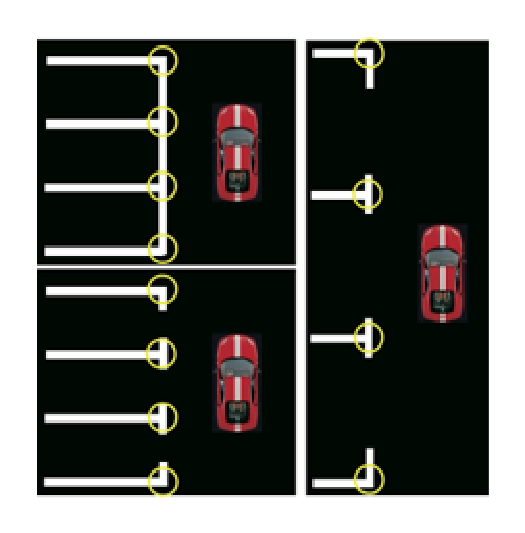
\includegraphics{pic/fig3_CNN_based_Parkinglot_Recognition}
% \caption{
% In this graph, yellow circles show the image patterns to be detected.\cite{Li2017Vision}
% }\label{fig:3}
% \end{figure}
% First, marking-point patterns are detected by a binary classifier. 
% Marking-point pattern refers to a image patch at the intersection of two parking-lines.
% \cite{Li2017Vision} The popular AdaBoost frame work is used. 
% A boosted classifier is made up of several weak classifiers, which, in our case, are shallow decision tree. 
% Three types of feature—— the normalized intensity, the gradient magnitude and the oriented gradient histograms are used. 
% Also, the “constant soft-cascade” strategy\cite{Li2017Vision} is introduced for acceleration. 
% Since there are five kinds of marking point patterns, there are five classifiers rather than one. 
% Once a marking-point pattern is detected, it is rotated to fit the standard pattern. 
% \begin{figure*}
% \centering
% 
\includegraphics[height = 1.6in]{pic/fig4_CNN_based_Parkinglot_Recognition}
% \caption{
% Examples of marking point patterns, the red arrow indicates the direction of each patterns.\cite{Li2017Vision}
% }\label{fig:4}
% \end{figure*}
% Parking lots are then recognized based on the marking-point patterns. 
% In this method, the entrance-line is especially focused. 
% We use the entrance-line rule to make preliminary detections. 
% A further decision is made by conforming the preliminary detection to the parking lot model.
% \begin{figure}
% \centering
% \includegraphics[height = 1.5in]{pic/fig5_CNN_based_Parkinglot_Recognition}
% \caption
%     In this figure,$\overrightarrow{{P}_{1}{P}_{3}},$ $\overrightarrow{{P}_{1}{P}_{2}}$ and $\overrightarrow{{P}_{2}{P}_{3}}$ consist three lots, but $\overrightarrow{{P}_{1}{P}_{3}}$ is a false positive detection.\citep{Li2017Vision}
% \label{fig:5}
% \end{figure}
% The final step is to remove the miss-detected entrance-line, like $\overrightarrow{{P}_{1}{P}_{3}}$in Fig 5.
%
%The raw detection results from the previous method are still not precise. 
We further optimize the results by firstly removing the entrance-line candidate who has more than two marking-point patterns on it to avoid this situation\COMMENT{what do u mean?}.  
Secondly, extremely large or small candidates are also discarded as all slots are around the same size.
Once a parking-line is detected, the direction of a lot is determined as well. 
And the “depth” of a parking lot is known a prior knowledge.\COMMENT{what do u mean?} 

%Since the relative car coordinate overlaps the top-view image coordinate, the slot coordinate in the top-view image is the same as that in the vehicle relative coordinate, and thus, we only need to perform a scale transformation.
%
%(John: ADD how to parameterize the parking slot, if we planned to optimize the shape of a parking slot? )
Since the corners of a parking slot are not fully observable.
To optimize a slot's shape as well as its position, a slot is represented by four points other than one.
Each point is connected with other three ones with a rectangular constrain(\Reffig(??)), which consists of an angular constraint of high confidence and a distance constraint with a relatively lower confidence.
The observation between four point of a slot and vehicle position is also applied to connect the slot to the global map.

%

ID of a parking slot is important for the association of this semantic landmark.
We fine tuned PVANet to detect each character in one ID \citep{Hong2016PVANet}.
The entrance-line of the parking slot is firstly utilized to roughly locate the ID, as shown in \Reffig(??).
Then the image patches are extracted and send to the CNN (\Reffig(??)).
Due to the distorted and blurred texture in the surround view image, even the latest detection network could not offer the satisfactory performance.
As a result, we devised a semantic-assisted association method to cope with the uncertainty, which will be detailed in \Refsec{sec:optimization}.  

% Lot IDs are also recognized basing on the priori knowledge of parking lots since IDs are always located in the center of the entrance-line. 
% We fine tuning the PVANet\cite{Hong2016PVANet} to detect IDs. 



% needed in second column of first page if using \IEEEpubid
%\IEEEpubidadjcol

\subsection{Visual fiducial marker localization}

The surround view system offers an intuitive ground observation at a high frame rate, however it has limitations. 
The visibility range and resolution of the top-view image is far from satisfactory, limiting the slot detection performance. 
% Most part of the surround view images are discarded, only downward parts are available. 
And the calibration for image fusion becomes inaccurate as time goes, which will deteriorate the slot measurement.

Recalling the goal of our robustly localization system for autonomous driving and parking in various parking lots, certain numbers of faithful landmarks such as visual fiducial markers still have to be incorporated.

\begin{figure}
\centering

\includegraphics{pic/fig6_Visual_markers}
\caption{An example of AprilTag}\label{fig:6}
\end{figure}

We adopted AprilTag and employed the detection framework from the AprilTag C source Open Library \footnote{https://april.eecs.umich.edu/wiki/AprilTags}\cite{Olson2011AprilTag}.
We further solved the relative position between visual markers and the vehicle by the PnP model in a fast and accurate way \cite{Hartley2003Multiple}. 

%\COMMENT{John: Can we improve the efficient or the accuracy when localization a tag?}
% Every tag texture indicates a unique ID, so tag data association is always correct.

\begin{figure}
\centering
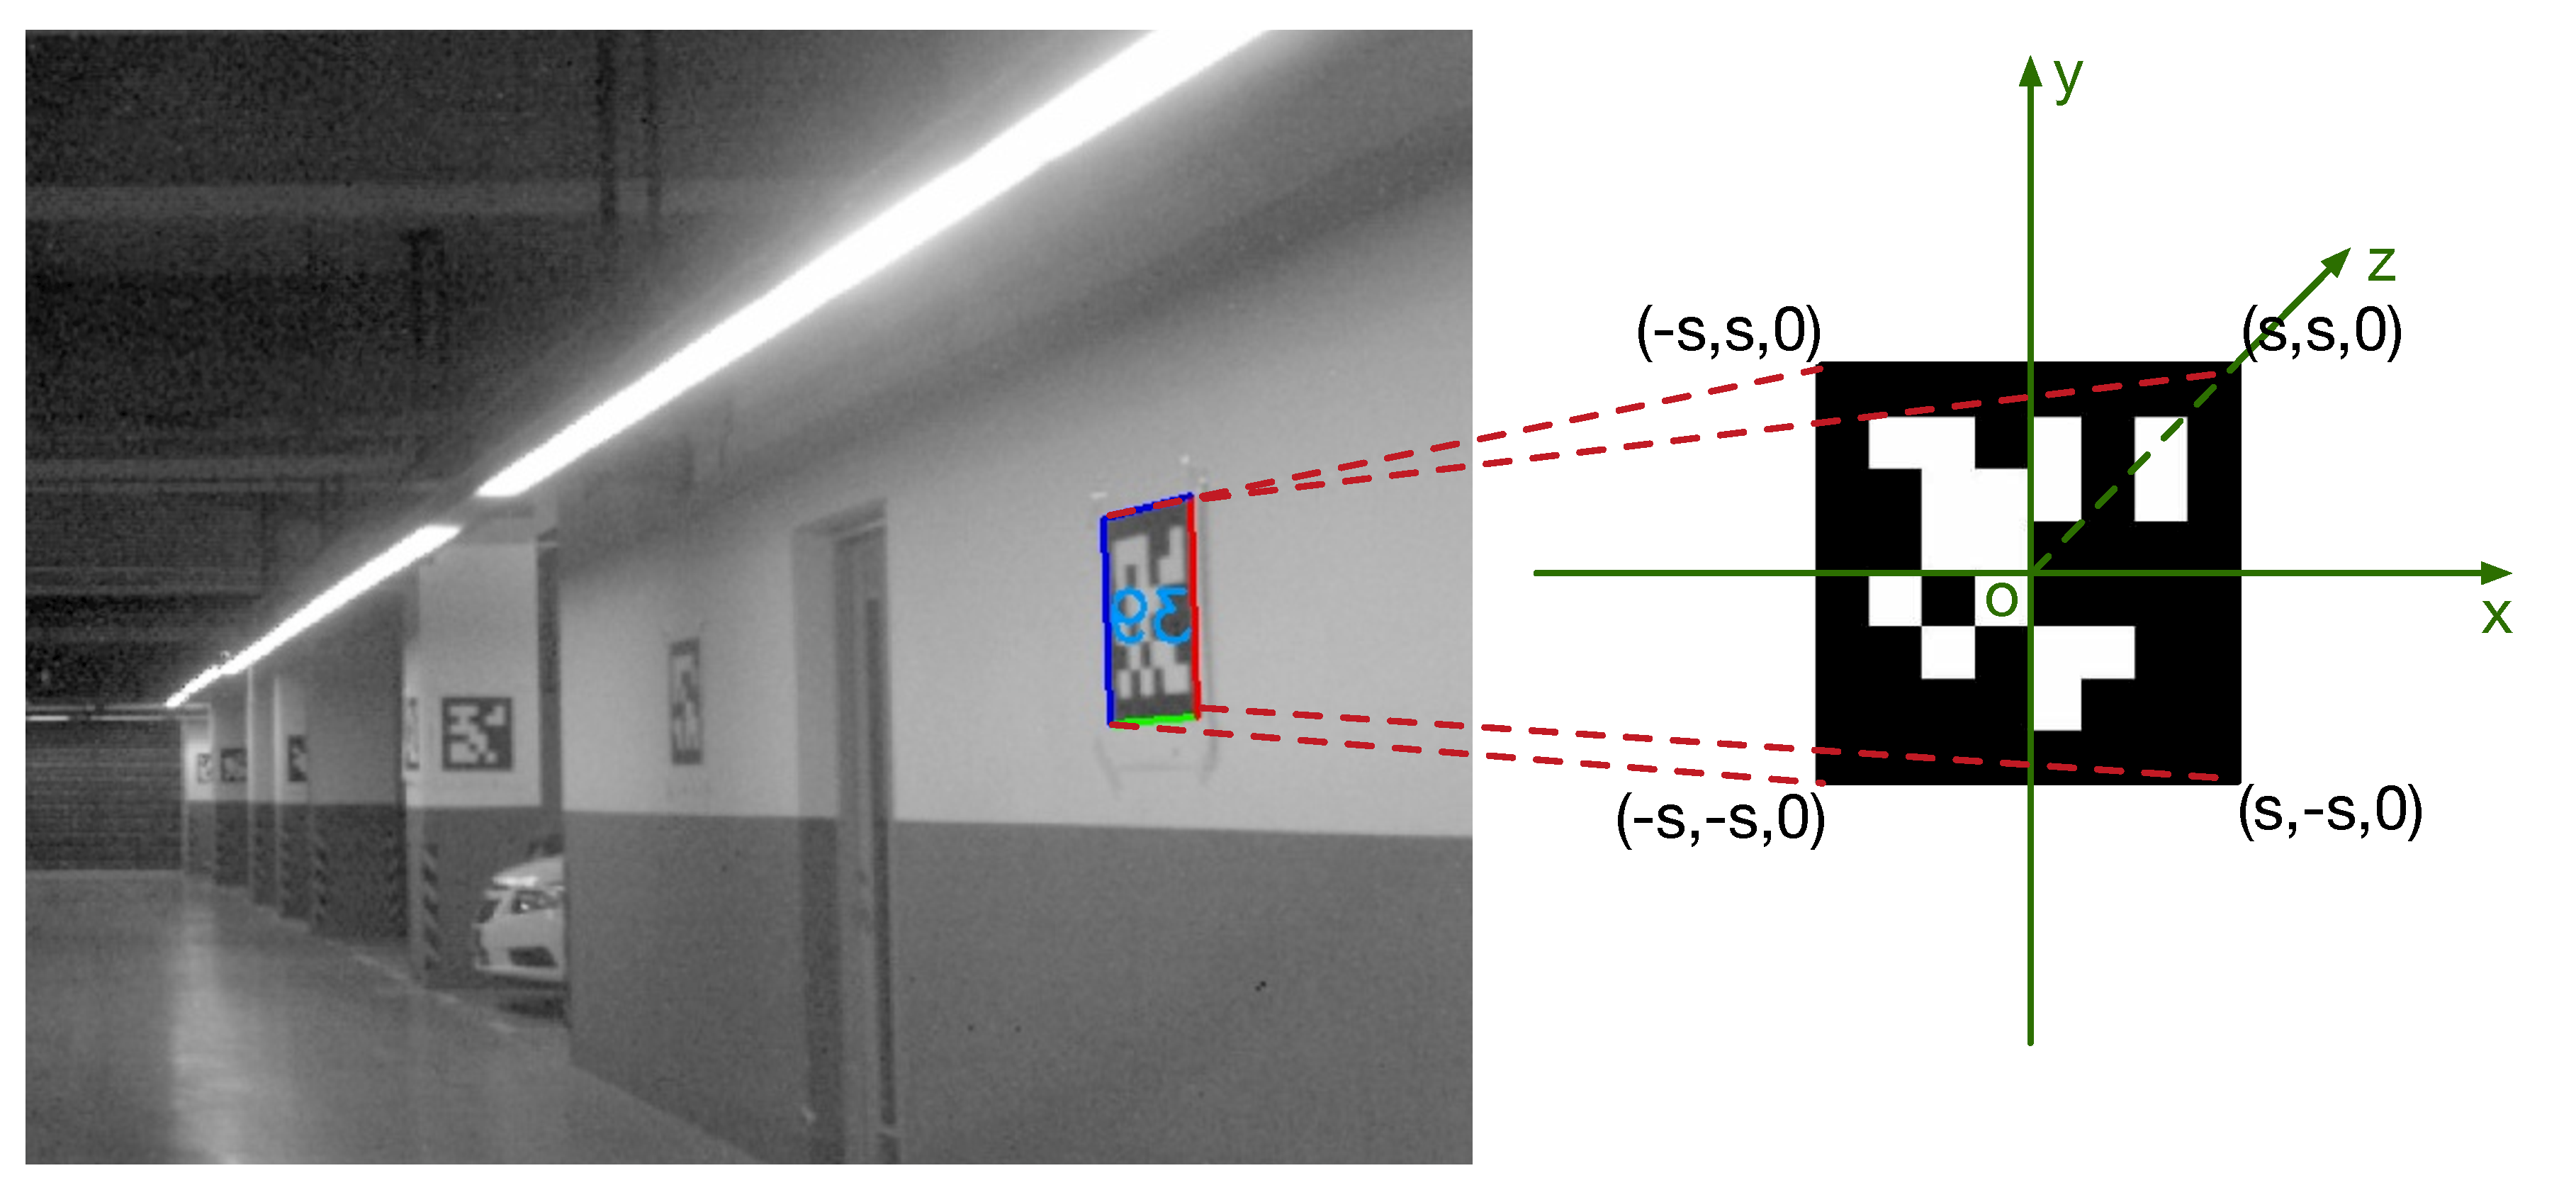
\includegraphics[height = 1.6in]{pic/fig7_Visual_markers}
\caption{
An example of the relationship between a detected tag in the image plane(left figure) and its corresponding hypothetical 3D tag coordinate(right figure)
}\label{fig:7}
\end{figure}

In the PnP model, we assume four corner points of the tag always lie on the same plane, and thus definite the hypothetical 3D tag coordinate(whose origin is a tag’s geometrical center, x axis and y axis are both parallel to tag’s edge, pointing rightward and upward respectively, and z axis is perpendicular to the tag plane, pointing inward). 
So the relationship between the tag corner in the image and that in the hypothetical 3D tag coordinate can be described as,
${R}_{3 \times 3} \cdot {{K}_{3 \times 3}}^{-1} \cdot {x}_{3 \times 1}+{t}_{3 \times 1}={X}_{3 \times 1}$
where ${R}_{3 \times 3}$ and ${t}_{3 \times 1}$ are the relative rotation and translation vector, 
${K}_{3 \times 3}$ is the intrinsic camera matrix, 
${X}_{3 \times 1}$ is the coordinate in the hypothetical 3D tag coordinate and ${x}_{3 \times 1}$ is the homogeneous coordinate in the image plane. 
%${X}_{3 \times 1}$ and ${K}_{3 \times 3}$ are prior knowledge, and ${x}_{3 \times 1}$ has already been detected. 
%Only ${R}_{3 \times 3}$ and ${t}_{3 \times 1}$ are unknown parameters with 6 DOF, more than 3 corresponding points are needed for iteration. 

%Once ${R}_{3 \times 3}$ and ${t}_{3 \times 1}$ is calculated, the Rodrigues transformation is performed on ${R}_{3 \times 3}$ to separate the angle($\alpha$) bonded by the array starts from the tag to the north and the array starts from the tag center to the vehicle. 
In the experiment, we find ${R}_{3 \times 3}$ given by PnP method is not accurate enough, since \COMMON{what...}
%cannot always meet our demands in accuracy.
So we discard ${R}_{3 \times 3}$ and get angle directly from the calibrated image.
As shown in(\Reffig(??)), the angle($\alpha$) can simply be calculated by $\alpha = \arctan((x_i - x_0) / f)$, where $x_i$ and $x_0$ denote the x coordinate value of the tag centre and the principle point respectively, and f is the focal length.
The distance($d$) is the 2-norm of ${t}_{3 \times 1}$ . 
So the tag locates at $( x=sin(a) \cdot d, y=cos(a) \cdot d)$ in the vehicle relative coordinate.

%

These visual fiducial markers are flexible and easily implemented.
They brought another benefit for the autonomous parking purpose, that fiducial markers can easily indicate the existences of pillars and walls which can only be robustly detected by expensive laser scanners.
These obstacle information can facilitate the route planning inside of a parking lot. 
% Pillar-walls are part and crucial in parking slots. 
% They can be used for localization, indoor structure inference and obstacle avoidance. 
% However, pillar-wall detections using image segmentation cost much time and still offer unstable results. 
% Though RGBD camera like Kinect can captures walls easily, they do cost a lot. 
% Visual markers, which present pillar-walls are introduced for its robustness and high efficiency.

\subsection{Optimization}
\label{sec:optimization}
\subsubsection{Optimization Pipeline}
we adopt a Graph-based optimization back-end.
However, due to fallible detection of parking slots and their ids from low-quality surround vision images, ambiguities will be presented during data association, which greatly affect the mapping and localization.
%False positives occur in both detection and data association of parking slots, and affect map and localization greatly.
%In front-end part, several methods have successfully lowered the slot detection error, while wrongly associated slots still cannot be detected.
Thus, correct association should be ensured and wrong ones should be detected and discarded in the optimization.
These are performed at both front-end and at back-end.
%error detection and fixation in slot detection and association should be performed in both front-end and back-end.

At every frame, parking slot observations are pre-associated through their ids and the nearest neighbour search.

\COMMENT{add association method by IDs, introducing some metric such as semantic distance?}

The nearest neighbour is based on the relative offsets between landmarks, which is derived 
%the relative car-landmark position(including the slots and visual markers), together with the speed and angular changes of vehicle are collected to the parking map incrementally. 
%These values are achieved 
from a Kalman-based extrapolator with the steering wheel, car speed and the compass readings from a cheap IMU as the inputs.

%

We further added the pre-associated landmarks into our graph model based on a Max-Mixture model\citep{Pfingsthorn2014Representing}.
% is therefore introduced and improved to not only detect but also correct mistaken associations.
%And 
The overall of the optimization pipeline is shown in \Reffig{fig:5}. 

\begin{figure}
\centering
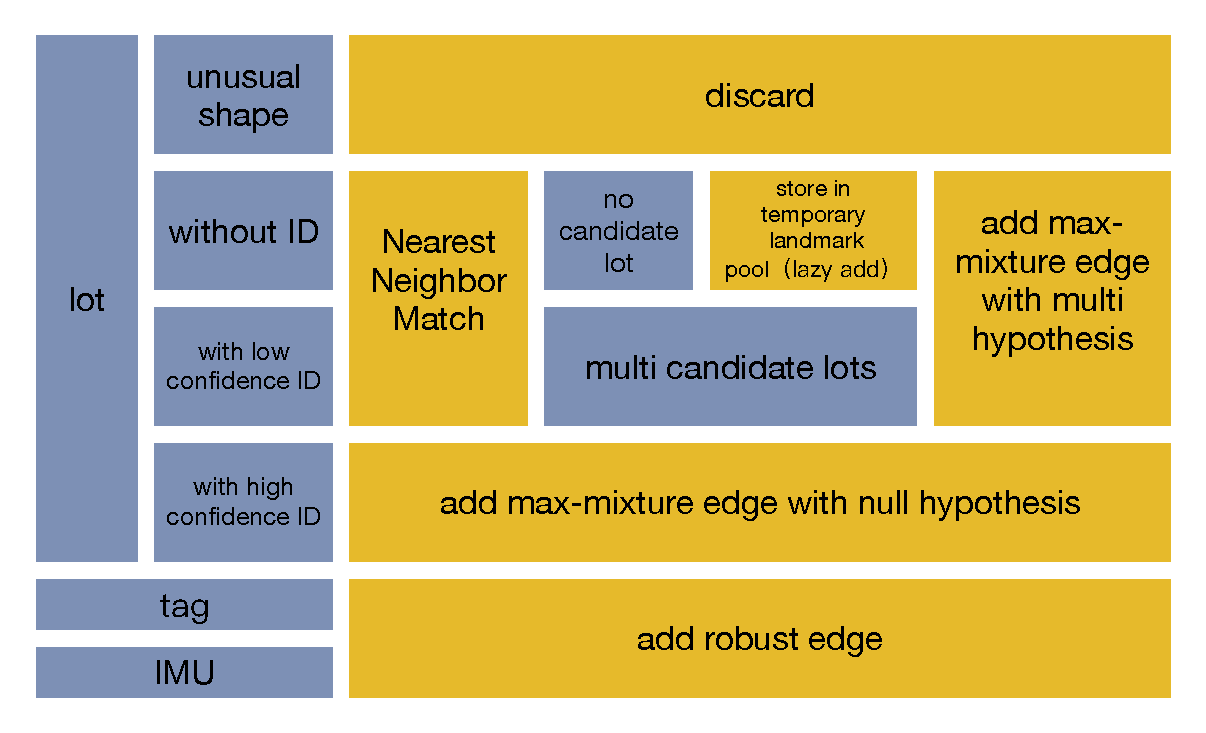
\includegraphics[height = 2.2in]{pic/fig8_Optimize}
\caption{
The overall pipeline of optimization
}\label{fig:5}
\end{figure}

\subsubsection{Optimization Framework}
% In this section, a map of parking slots is built by fusing all the observation datum collected in the former sections. 
% The accumulated error of IMU may cause drifting in localization. 
% To avoid these problems, we use the popular g2o\cite{K2011G2o} framework together with the max-mixture model \cite{Pfingsthorn2014Representing} to optimize both car and landmarks positions and ensure correct data association in the offline section, the figure above give the overall view of the optimization step.
We adopted G2O \citep{K2011G2o} in our method.
%offers a global framework for nonlinear least square problems. 
%Under the G2O framework, 
%All the elements to be optimized are regarded as vertices, while all the observation constraints are known as edges who connect vertices. 
%In our method all the observations of parking slots and fiducial markers are treated as edges in the graph. 
% Observations from vehicle to tag or vehicle are presented by G2O standard edges. 
%However, ambiguity raised from observations of parking slots as well as parking ids lead to erroneous data associations and generate fatal residual error in the optimization. 

%Several robust optimization extensions exist, in the paper, max mixture models\citep{Pfingsthorn2014Representing} are introduced to detect and eliminate the mistaken associations.
% ID detection error is inevitable, so max mixture models \cite{Pfingsthorn2014Representing} are 
% introduced to eliminate the mistaken associations.
The least square problem of graph optimization can be expressed by the following equation:
\[
F(x)=\sum\limits_{k \in C}e_k{(x_k,z_k)}^T{\Omega}_k e_k(x_k,z_k)
\]
\[
x^{*} = \mathop{argminF(x)}\limits_x
\]
where $C$ denotes the total ID group; 
$x_k$is the parameter block of the $k$Th vertex(containing the vertex’s location and direction), $z_k$ and $\Omega_k$ is the mean and covariance of the $k$Th edge; 
$e_k(x_k,z_k)$ measures how well $x_k$ matches $z_k$. 
These elements consist the global error function $F(x)$ , and $x^*$ is the global optimal solution.
%To find the solution $x^*$, $F(x)$ is rewrote as $F(\check{x}+\Delta x)\simeq c+2b^T \Delta x + \Delta x^T H \Delta x$, 
%while $c=\sum\limits_{k \in C}e_k^T \Omega_k e_k$; 
%$b=\sum\limits_{k \in C}e_k^T \Omega_k J_k$; 
%$H=\sum\limits_{k \in C}J_k^T \Omega_k J_k$; 
%$\check{x}$ indicates the initial value of ${x}$. 
%$\Delta x$ is the residual between $\check{x}$  and $x^*$, and $J_k$ is the Jacobian Matrix of %each $e_k$. 
%Then we can get the global optimal solution $x^*$ by solving the linear function $H\Delta x^*=-b$ and add $\Delta x^*$ to $x^*$ iteratively.

We can get $x^*$ by solving the linear function iteratively, and the uncertainties of $z_k$ are described by noise models who are uni-model Gaussian. 
This classical graph framework works quite well when there are only visual markers and IMU measurements in parking map, but it gives bad results once parking slots are added.
Since every parking slots may be wrongly associated or detected, it's impractical to measure their noises by a single model. 

%Finally, all the detected ID and measurement of parking lots are added to the graph as max mixture \cite{Pfingsthorn2014Representing} edges with multiple hypothesis including null hypothesis.
%

%We propose to additionally feed the offline optimized map as the initialization for online extended Kalman filter (EKF) framework.
%The reason is the performance of graph-based optimization is inferior to EKF during online localization applications.
% Thus, the offline part outputs a 2D parking map and an optimized vehicle trajectory. 
% During the online stage, the former parking map acts as the initial map, and is updated simultaneously with the extended Kalman filter(EKF). 
% This results in a smoother trajectory, which helps the further control task.

%\COMMENT{Yewei: highlight, comparing to the traditional methods, why semantic, how outliers}

\subsubsection{Outliers elimination using Max-Mixture Model}
As mentioned above, classical graph optimization method using uni-model Gaussian is sensitive to outliers, and fails when there are wrongly associations in graphs.
Several robust methods\citet{maxmixture} \citet{Switchable Constrain} \citet{RRR} have been proposed for the pose graph.
In this paper, we apply the Max-mixture model to both poses and landmark positions.
\COMMENT{john: why the max mixture model is used? because of its simplicity?}

%

This model describes observation ambiguities as multi-model Gaussian, thus wrongly associated data can be suppressed by other mixture elements. 
To simplify the problem, the sum is substituted by a max operator. 
In this paper, when an uncertain loop closure is detected, a Max-Mixture of all possible loop closure alternatives and a null hypothesis is thus added to the graph.

\COMMENT{1 how to evaluate uncertainty}
\COMMENT{2 how to detect incorrect associations}
\COMMENT{3 how to eliminate incorrect associations}
%several possible loop closure alternatives and a null hypothesis indicating that all the former alternatives are wrong. 
Semantics attached to landmarks, the slot IDs, are used.... . 
%

%Max-Mixture model share some similarities with slot ambiguity, so it can help fix data association problem and to some extent, implement semantic information.
%Max-Mixture Model aims to detect loop closure errors in the “back-end” part of a pose graph. 
%Traditionally, all distributions in a “back-end” graph system are considered as unimodal Gaussians, thus wrongly associated datum result in great global errors. 
%When sum-mixture model replaces unimodal Gaussian, wrongly associated data can be suppressed by other mixture elements. 
%Observation noises are described by multi-model Gaussian, thus wrongly associated data can be suppressed by other mixture elements. 
%To simplify the problem, the sum is substituted by a max operator. 
%In the pose graph situation, when an uncertain loop closure occurs, a Max-Mixture of several elements is thus added to the graph: several possible loop closure alternatives and a null hypothesis indicating that all the former alternatives are wrong. 
%In the parking map with loop closures triggered by observing a pre-visited landmark, Max-Mixture still works.
%A null hypothesis is quite effective even with a extremely small weight.\cite{Pfingsthorn2014Representing}  
%This method works well in pose graphs\cite{Latif2014Robust}\cite{Sunderhauf2013Switchable}\cite{Cadena:2016fp}, and we will prove its effectiveness in landmark association in the experiment section.

%Since there is no wrongly associated data in IMU and tag observations, they are considered as robust edges in the graph, while the parking lot observations are always with high uncertainty, and several steps are added to guarantee the robustness. 
%Once parking lots are detected, they are re-examined using some prior knowledge. 
%Unusual lots(too small, too large or with abnormal length-width ratio) will thus be discarded. 
Since the shapes of parking slots are similar to each other, we evaluate the uncertainty of loop closure based on IDs and their poses.


Only noises of parking slots are treated as multi-model Gaussian, while in other situations, uni-model Gaussian is enough.
After the elimination based on prior knowledge in front-end, slots are classified by the confidence level of lot ID detections. Lot observations with high confidence IDs are added to the graph as Max-Mixture edges with null hypothesis. 
A null hypothesis is always essential due to the existence of false positive ID detection results with high confidence. 
The rest slots get several data association hypothesis by processing nearest neighbour search in the existing parking map.  
These candidate hypothesis together with the original hypothesis obtained by lot detection result consist a Max-Mixture landmark observation element with multi hypothesis. 
This element is then added to the graph, only one hypothesis will be selected during optimization.
A new landmark hypothesis will not be added to the map until it is repeatedly observed for a certain number of time. 
When slot ID detection only achieves partially success(only one in two digits is detected), Max-Mixture can also help decide the full slot ID.
%The best car lot association will be selected as the initial landmark observation.
Inspired by \citep{Switchable constraints}, information matrix of landmark edges are shifted according to their detection confidence level.

%The vertices collection of the graph includes vehicle position at every time stamp and all landmark(tags and lots) positions. 
%The graph is optimized by Gauss-Newton Method once a new landmark edge is added. All the optimized landmarks consists of the initial 2D map.

%In the online part, the well-known Extended Kalman Filter(EKF)\cite{Bailey2006Simultaneous} is introduced to filter the inconsistency in localization results from various observation. 

%\subsubsection{Extended Kalman Filter--trash}
%Extended Kalman Filter\cite{Bailey2006Simultaneous}is a classical “back-end” choice in SLAM field. 
%Since there are errors in all the observations, EKF is used to determine to which extent the observations can be believed. 
%The following equations express the whole optimization procedure:
%$
%{\hat x}_{k|k-1}=f({\hat x}_{k-1|k-1},{u}_{k-1})\\
%{P}_{k|k-1} = {F}_{k-1}{P}_{k-1|k-1}{F}_{k-1}^{T}+{Q}_{k-1}\\
%\\
%{\widetilde y}_{k}={z}_{k}-h({\hat x}_{k|k-1})\\
%{S}_{k}={H}_{k}{P}_{k|k-1}{H}_{k}^{T}+{R}_{k}\\
%{K}_{k}={P}_{k|k-1}{H}_{k}^{T}{S}_{k}^{-1}\\
%{\hat x}_{k|k}={\hat x}_{k|k-1}+{K}_{k}{\widetilde y}_{k}\\
%{P}_{k|k}=(I-{K}_{k}{H}_{k}){P}_{k|k-1}\\
%$
%\\
%$x$is the state matrix(containing real-time car pose and positions of all landmarks);  
% ${\hat x}_{k|k-1}$denotes the  calculated from the former state, ${\hat x}_{k-1|k-1}$ while denotes the former state matrix.  
% $z_k$ denotes the observations at k time stamp, 
% and $u_{k-1}$ is the control matrix(indicating IMU datum and real-time control of the vehicle control system). 
% $P$ is the corresponding covariance matrix of $x$, while $F_{k-1}$ and $H_k$ are the Jacobian matrix of $f({\hat x}_{k-1|k-1},{u}_{k-1})$ and $h({\hat x}_{k|k-1})$. 
% Both $Q$ and $R$ are pre-given noise matrix. Once updated, the state and covariance matrix are switched to fit current time stamp’s observations.

%We discard the graph optimization method to attain a smoother vehicle localization trace, which is meaningful for the later control part. 
%Except for lot and tag observations, the car direction and speed from both IMU and vehicle control system (the steering wheel) are also added to the filter. 
%This combination enables a more robust localization performance in various harsh situations(etc. long term localization under limited tags or lots with large direction drifting in IMU, which is discussed in the Experiments part). 
%Since the covariance matrix increases quadratically with the number of landmark\cite{Bailey2006Simultaneous}, local map is introduced to achieve real-time performance. 
%Those landmarks who has not been observed for a period of time is removed from the local map. 
%The online localization can start from either an empty map or the initial parking map built in the offline stage. 
%However, due to the local map strategy, the online lot map starting from an empty map is to improved.

\begin{figure}
\centering
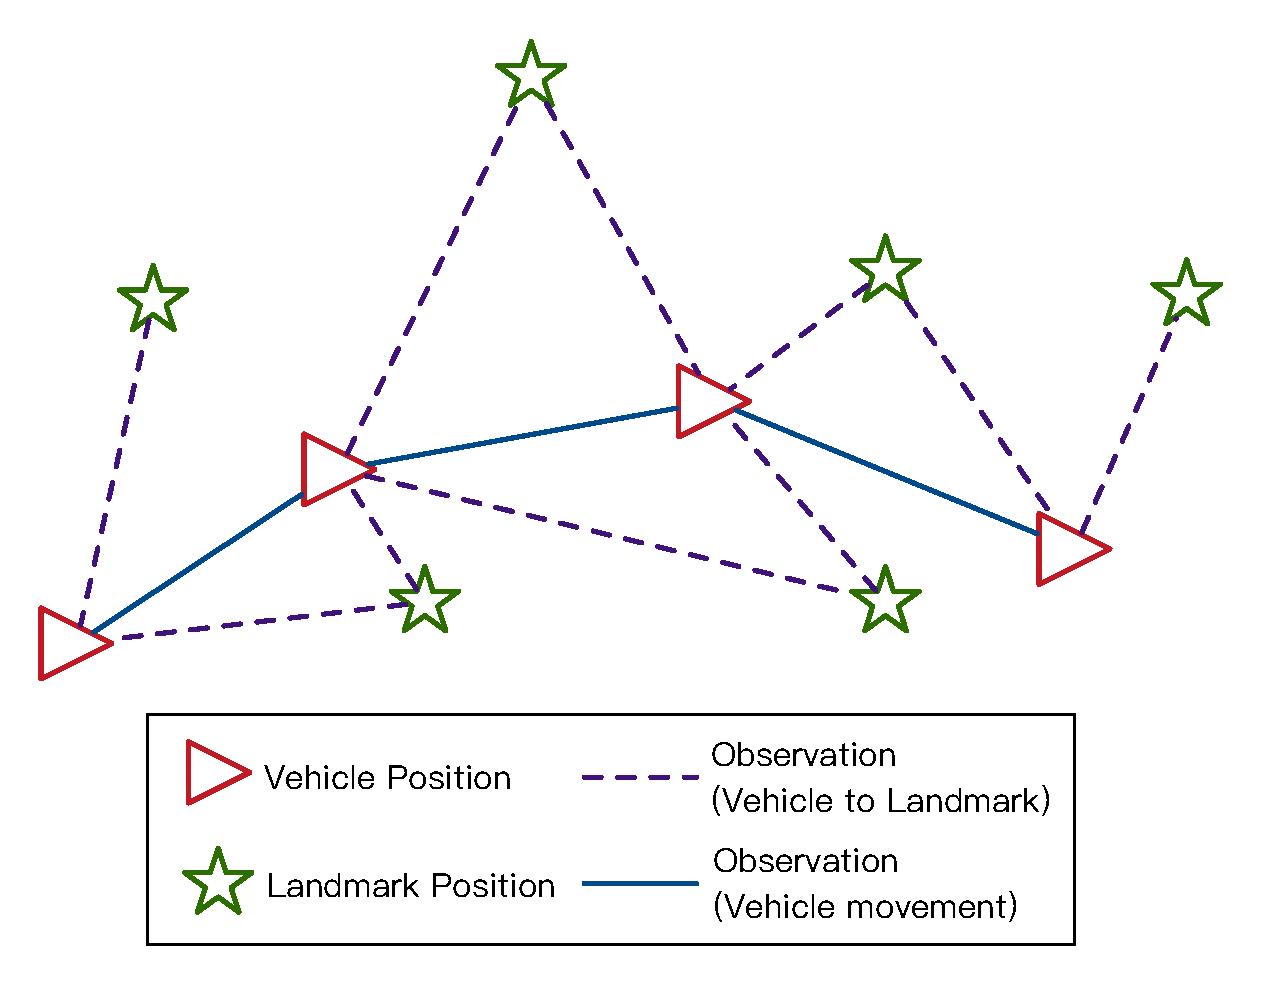
\includegraphics[height = 2.2in]{pic/fig9_Optimize}
\caption{
The connection between the vehicle at each time stamp and the landmarks.
}\label{fig:9}
\end{figure}



\section{Experiments}
\COMMENT{JOHN: should firstly describe the test environment, size map lighting condition and car etc.}
\COMMENT{How outliers detection successful?}

In this section, we test our method both online and offline, and discuss several questions about the usage of visual markers. 
All the parking lot datasets are collected and tested by TiEV autonomous vehicle \footnote{cs1.tongji.edu.cn/tiev} .
\subsection{Semantic landmark detection and localization}

\COMMENT{John: models used, training workflow, training samples and detection results and statistics, short conclusion}
\Reffig{??} show a subset of the training samples used.

\COMMENT{John: offline should be placed before online}

\subsection{Offline mapping test}
As to the offline part, several datasets with different starting points are collected. 
Each dataset is processed independently.
The covariance of each edge shifts from 0.1 to 0.25 according to its confidence level.
Fig 12 shows the map result for two of these datasets.
Map blocks with more tags have higher precision as tags are ideal landmarks who will never be wrongly associated.
The low detection rate of parking ID also affects the mapping result, as shown in fig 13.

\begin{figure*}
\centering
%\includegraphics[height = 1.2in]{pic/404}
\caption{
toDo%有tag的建好的图,标出无tag部分,loop closure前后的图,共四个
}\label{fig:12}
\end{figure*}

\begin{figure*}
\centering
%\includegraphics[height = 1.2in]{pic/404}
\caption{
toDo%有tag的parking ID经过调整和未经过调整的图,两对,共四个
}\label{fig:13}
\end{figure*}

In one dataset, there is a no-tag map block (marked in fig 12), where wrongly associated data always occurs.
However, once a loop is detected, all landmark-positions are corrected.
Then, duplicate landmarks are merged.

\subsection{Online real-time mapping and localization}
During the online part, the vehicle is first operated by human to initialize the parking map. 
Once the map stabilizes, a car trace is recorded.
Then the vehicle drives automatically at the speed of 3 km/h following this pre-recorded trace and fixes its direction constantly according to real-time localization record.
The automatic driving procedure is repeated 10 times, automatic driving traces are also recorded and compared to the pre-recorded one.
Fig 11 shows the traces of both manual and automatic driving trace.
Quite a number of visual markers(60 tags) are used to cover the lot-free parts near the entrance and to guarantee a fully stable and credible localization result.
Each tag is printed on a A2-size paper with 48.8 cm side length.
While observing, those tags who are 20 meters or farther than the vehicle are discarded since the accuracy decreases as tags become smaller in the image.
However, observations with dip-angle are reliable constraints as long as they are within 20 meters.

\begin{figure}[htbp]
\centering
%\includegraphics[height = 1.2in]{pic/404}
\caption{
The dip-angle doesn't affect the accuracy while the distance makes great influence.%想用立体的效果来表示,不知道该如何表示?
}\label{fig:10}
\end{figure}

\begin{figure}[htbp]
\centering
%\includegraphics[height = 1.2in]{pic/404}
\caption{
A comparison between the human-driving and automatic driving trace%这个数据是否可以再采集一次?
}\label{fig:11}
\end{figure}

\subsection{Comparison with ORB2-SLAM}

\subsection{How many tag is needed?}

As described in the previous section, tags are ideal landmarks promising a robust localization and mapping result.
In this part, we discuss which tags are indispensable while others are not a must.

We think several factors may affect the importance of each tag: the visibility rate, the distribution and the distance to the nearest rate.
Considering the factors above, we make several tag combinations and test their performance.
The final result is shown in fig 14, both visibility and distribution play an important role.
The crucial tags should be separated in the lot, and have a good visibility rate.
In our parking lot case, at least 3 tags are needed, while 10 evenly distributed tags offer the best result.

\begin{figure*}
\centering
%\includegraphics[height = 1.2in]{pic/404}
\caption{
toDo%tag数量和分布不同的图
}\label{fig:14}
\end{figure*}

$\\
\\$

a statistic result of the rightly located lots in each graph
give the  tag position solution based on the visibility of cameras
based on visibility of the front camera(put tags at where there are multi visibility)
be separated in the lot
compare the solution to the statistic result
very similar

\COMMENT{John: should add Tags can be replaced by instruction arrows or parkinglot ids on the pillar, here restricted by the goal and the environment tags are required }
% An example of a floating figure using the graphicx package.
% Note that \label must occur AFTER (or within) \caption.
% For figures, \caption should occur after the \includegraphics.
% Note that IEEEtran v1.7 and later has special internal code that
% is designed to preserve the operation of \label within \caption
% even when the captionsoff option is in effect. However, because
% of issues like this, it may be the safest practice to put all your
% \label just after \caption rather than within \caption{}.
%
% Reminder: the "draftcls" or "draftclsnofoot", not "draft", class
% option should be used if it is desired that the figures are to be
% displayed while in draft mode.
%
%\begin{figure}[!t]
%\centering
%\includegraphics[width=2.5in]{myfigure}
% where an .eps filename suffix will be assumed under latex, 
% and a .pdf suffix will be assumed for pdflatex; or what has been declared
% via \DeclareGraphicsExtensions.
%\caption{Simulation results for the network.}
%\label{fig_sim}
%\end{figure}

% Note that the IEEE typically puts floats only at the top, even when this
% results in a large percentage of a column being occupied by floats.


% An example of a double column floating figure using two subfigures.
% (The subfig.sty package must be loaded for this to work.)
% The subfigure \label commands are set within each subfloat command,
% and the \label for the overall figure must come after \caption.
% \hfil is used as a separator to get equal spacing.
% Watch out that the combined width of all the subfigures on a 
% line do not exceed the text width or a line break will occur.
%
%\begin{figure*}[!t]
%\centering
%\subfloat[Case I]{\includegraphics[width=2.5in]{box}%
%\label{fig_first_case}}
%\hfil
%\subfloat[Case II]{\includegraphics[width=2.5in]{box}%
%\label{fig_second_case}}
%\caption{Simulation results for the network.}
%\label{fig_sim}
%\end{figure*}
%
% Note that often IEEE papers with subfigures do not employ subfigure
% captions (using the optional argument to \subfloat[]), but instead will
% reference/describe all of them (a), (b), etc., within the main caption.
% Be aware that for subfig.sty to generate the (a), (b), etc., subfigure
% labels, the optional argument to \subfloat must be present. If a
% subcaption is not desired, just leave its contents blank,
% e.g., \subfloat[].


% An example of a floating table. Note that, for IEEE style tables, the
% \caption command should come BEFORE the table and, given that table
% captions serve much like titles, are usually capitalized except for words
% such as a, an, and, as, at, but, by, for, in, nor, of, on, or, the, to
% and up, which are usually not capitalized unless they are the first or
% last word of the caption. Table text will default to \footnotesize as
% the IEEE normally uses this smaller font for tables.
% The \label must come after \caption as always.
%
%\begin{table}[!t]
%% increase table row spacing, adjust to taste
%\renewcommand{\arraystretch}{1.3}
% if using array.sty, it might be a good idea to tweak the value of
% \extrarowheight as needed to properly center the text within the cells
%\caption{An Example of a Table}
%\label{table_example}
%\centering
%% Some packages, such as MDW tools, offer better commands for making tables
%% than the plain LaTeX2e tabular which is used here.
%\begin{tabular}{|c||c|}
%\hline
%One & Two\\
%\hline
%Three & Four\\
%\hline
%\end{tabular}
%\end{table}


% Note that the IEEE does not put floats in the very first column
% - or typically anywhere on the first page for that matter. Also,
% in-text middle ("here") positioning is typically not used, but it
% is allowed and encouraged for Computer Society conferences (but
% not Computer Society journals). Most IEEE journals/conferences use
% top floats exclusively. 
% Note that, LaTeX2e, unlike IEEE journals/conferences, places
% footnotes above bottom floats. This can be corrected via the
% \fnbelowfloat command of the stfloats package.




\section{Conclusion}
The conclusion goes here.





% if have a single appendix:
%\appendix[Proof of the Zonklar Equations]
% or
%\appendix  % for no appendix heading
% do not use \section anymore after \appendix, only \section*
% is possibly needed

% use appendices with more than one appendix
% then use \section to start each appendix
% you must declare a \section before using any
% \subsection or using \label (\appendices by itself
% starts a section numbered zero.)
%


\appendices
\section{Proof of the First Zonklar Equation}
Appendix one text goes here.

% you can choose not to have a title for an appendix
% if you want by leaving the argument blank
\section{}
Appendix two text goes here.


% use section* for acknowledgment
\section*{Acknowledgment}


The authors would like to thank...

% Can use something like this to put references on a page
% by themselves when using endfloat and the captionsoff option.
\ifCLASSOPTIONcaptionsoff
  \newpage
\fi


\bibliographystyle{IEEEtran}
\bibliography{slam_tiev}

% that's all folks
\end{document}